\section{Methodology}
\label{sec:methodology}

% ── Instructions ─────────────────────────────────────────────────────────
% This is the core technical section. Use subsections as below.
% Every equation should be numbered. Reference every figure and table.
% ─────────────────────────────────────────────────────────────────────────

\subsection{Notation}

We formulate the problem on a pose graph
$\mathcal{G} = (\mathcal{V}, \mathcal{E})$, where vertices represent poses
and edges represent spatial constraints.
The vertex set is partitioned into robot poses
$\mathcal{V}_{\mathrm{r}} = \{\mathbf{x}_t\}$ and anchor poses
$\mathcal{V}_{\mathrm{a}} = \{\mathbf{x}_{\mathcal{C}_i}\}$.
Both robot poses and camera poses are optimisation variables in the augmented
graph. Each robot state $\mathbf{x}_t \in SE(2)$ denotes the robot pose at
time index $t$, and each $\mathbf{x}_{\mathcal{C}_i} \in SE(2)$ denotes the
map-frame pose of infrastructure camera $\mathcal{C}_i$.
The edge set is partitioned into pose-pose constraints
$\mathcal{E}_{\mathrm{pp}}$ and pose-anchor constraints
$\mathcal{E}_{\mathrm{pa}}$.
In our case,
$\mathcal{E}_{\mathrm{pp}} = \mathcal{E}_{\mathrm{odom}} \cup \mathcal{E}_{\mathrm{loop}}$
contains odometry and loop-closure edges, and
$\mathcal{E}_{\mathrm{pa}} = \mathcal{E}_{\mathrm{cam}}$
contains camera-derived anchor edges.
Each edge carries a relative measurement
$\mathbf{z}_{ij}$ or $\mathbf{z}_{ik}$ and an associated information matrix.
For a residual vector $\mathbf{r}$ weighted by information matrix
$\boldsymbol{\Omega}$, we use the notation
$\|\mathbf{r}\|^2_{\boldsymbol{\Omega}} =
\mathbf{r}^{\top} \boldsymbol{\Omega} \mathbf{r}$.

\subsection{Pose-Graph Preliminaries}

Pose-graph SLAM can be viewed as a weighted directed graph
$\mathcal{G} = (\mathcal{V}, \mathcal{E}, \omega)$, in which each pose node
belongs to $\mathcal{V}$ and each edge in $\mathcal{E}$ encodes a relative
measurement between two poses~\cite{chen2022anchor}.
For the robot trajectory, let
$\mathcal{V}_{\mathrm{r}} = \{\mathbf{x}_1, \ldots, \mathbf{x}_{n_p}\}$
denote the set of $n_p$ robot poses and let
$\mathcal{E}_{\mathrm{pp}} = \{e_k\}_{k=1}^{m}$ denote the set of $m$
pose-pose constraints.
Each edge $e_k = (i,j)$ carries a relative measurement
$\mathbf{z}_{ij}$ and a positive weight $\omega_k > 0$, whose magnitude is
inversely related to the measurement variance and therefore reflects the
reliability of that constraint.

The graph structure can be encoded by the incidence matrix
$A \in \{-1,0,1\}^{n_p \times m}$.
For edge $e_k = (i,j)$, the $k$-th column of $A$ has entry $-1$ in row $i$,
+1 in row $j$, and zeros elsewhere.
If the edge weights are collected in the diagonal matrix
$W = \mathrm{diag}(\omega_1, \ldots, \omega_m)$, then the weighted graph
Laplacian is

\begin{equation}
    L_w = A W A^{\top}.
    \label{eq:weighted_laplacian}
\end{equation}

This matrix captures both graph topology and measurement confidence, and it is
useful for analyzing how strongly the pose graph is constrained.

In the multiple-anchor setting, a subset of nodes is designated as anchors.
In our formulation, the infrastructure cameras form the anchor-node set
$\mathcal{V}_{\mathrm{a}} = \{\mathbf{x}_{\mathcal{C}_i}\}$.
Removing the rows of $A$ that correspond to anchored nodes yields a reduced
incidence matrix $A_{\setminus \mathcal{V}_{\mathrm{a}}}$, and the
corresponding reduced weighted Laplacian becomes

\begin{equation}
    L_{w,\setminus \mathcal{V}_{\mathrm{a}}} =
    A_{\setminus \mathcal{V}_{\mathrm{a}}}
    W
    A_{\setminus \mathcal{V}_{\mathrm{a}}}^{\top}.
    \label{eq:reduced_laplacian}
\end{equation}

This viewpoint clarifies why anchor placement matters: informative anchors alter
the reduced graph structure and improve the observability of the remaining
unanchored robot poses.
In our case, camera detections provide pose-anchor measurements
$\mathbf{z}_{ik}$ between robot pose $\mathbf{x}_i$ and anchor pose
$\mathbf{x}_{\mathcal{C}_k}$, which are incorporated alongside the standard
pose-pose constraints.

Let $\mathbf{X} = \{\mathbf{x}_t\}$ denote the robot trajectory and
$\mathbf{C} = \{\mathbf{x}_{\mathcal{C}_i}\}$ the set of camera poses to be
optimized jointly.
The backend solves the nonlinear least-squares problem

\begin{equation}
    \begin{aligned}
        (\mathbf{X}^{\star}, \mathbf{C}^{\star}) =
        \arg\min_{\mathbf{X},\mathbf{C}} \;&
        \sum_{(i,j) \in \mathcal{E}_{\mathrm{pp}}}
        \|\mathbf{r}_{ij}(\mathbf{x}_i, \mathbf{x}_j; \mathbf{z}_{ij})\|^2_{\boldsymbol{\Omega}_{ij}} \\
        &+ \sum_{(i,k) \in \mathcal{E}_{\mathrm{pa}}}
        \|\mathbf{r}^{\mathrm{a}}_{ik}(\mathbf{x}_i, \mathbf{x}_{\mathcal{C}_k}; \mathbf{z}_{ik})\|^2_{\boldsymbol{\Omega}_{ik}}.
    \end{aligned}
    \label{eq:pose_graph_objective}
\end{equation}

The first term corresponds to the standard LiDAR SLAM objective over robot
poses, while the second term adds pose-camera constraints that connect robot
poses to persistent infrastructure nodes.
In the proposed method, each camera is represented by one node that is reused
across all of its detections, and each visual detection of the robot
contributes one pose-anchor edge.
These additional terms couple distant parts of the trajectory through the same
camera nodes and therefore counteract drift in sparse, repetitive, or
featureless environments without requiring a separate post-hoc registration of
camera locations onto an already drifted map.

\subsection{System Overview}

Figure~\ref{fig:system_overview} shows the overall workflow of the proposed
camera-augmented pose-graph SLAM system.
The robot runs a graph-based 2D LiDAR SLAM backend.
A set of $N$ ceiling- or wall-mounted cameras
$\{\mathcal{C}_i\}_{i=1}^{N}$ observe the workspace from stable viewpoints.
Unlike a post-processing pipeline in which cameras are first aligned to a
finished SLAM map, the proposed method inserts each camera directly into the
pose graph as a persistent node whose map-frame pose is refined jointly with
the robot trajectory.
A YOLO-based inference node~\cite{ultralytics2023} runs on each camera
stream; when the robot is detected, the node calls the
\texttt{add\_camera\_constraint} service to either initialise or update the
corresponding camera node and inject a factor into the Ceres pose graph,
thereby augmenting Eq.~\ref{eq:pose_graph_objective} with repeated
camera-to-robot observations.

\begin{figure}[t]
    \centering
    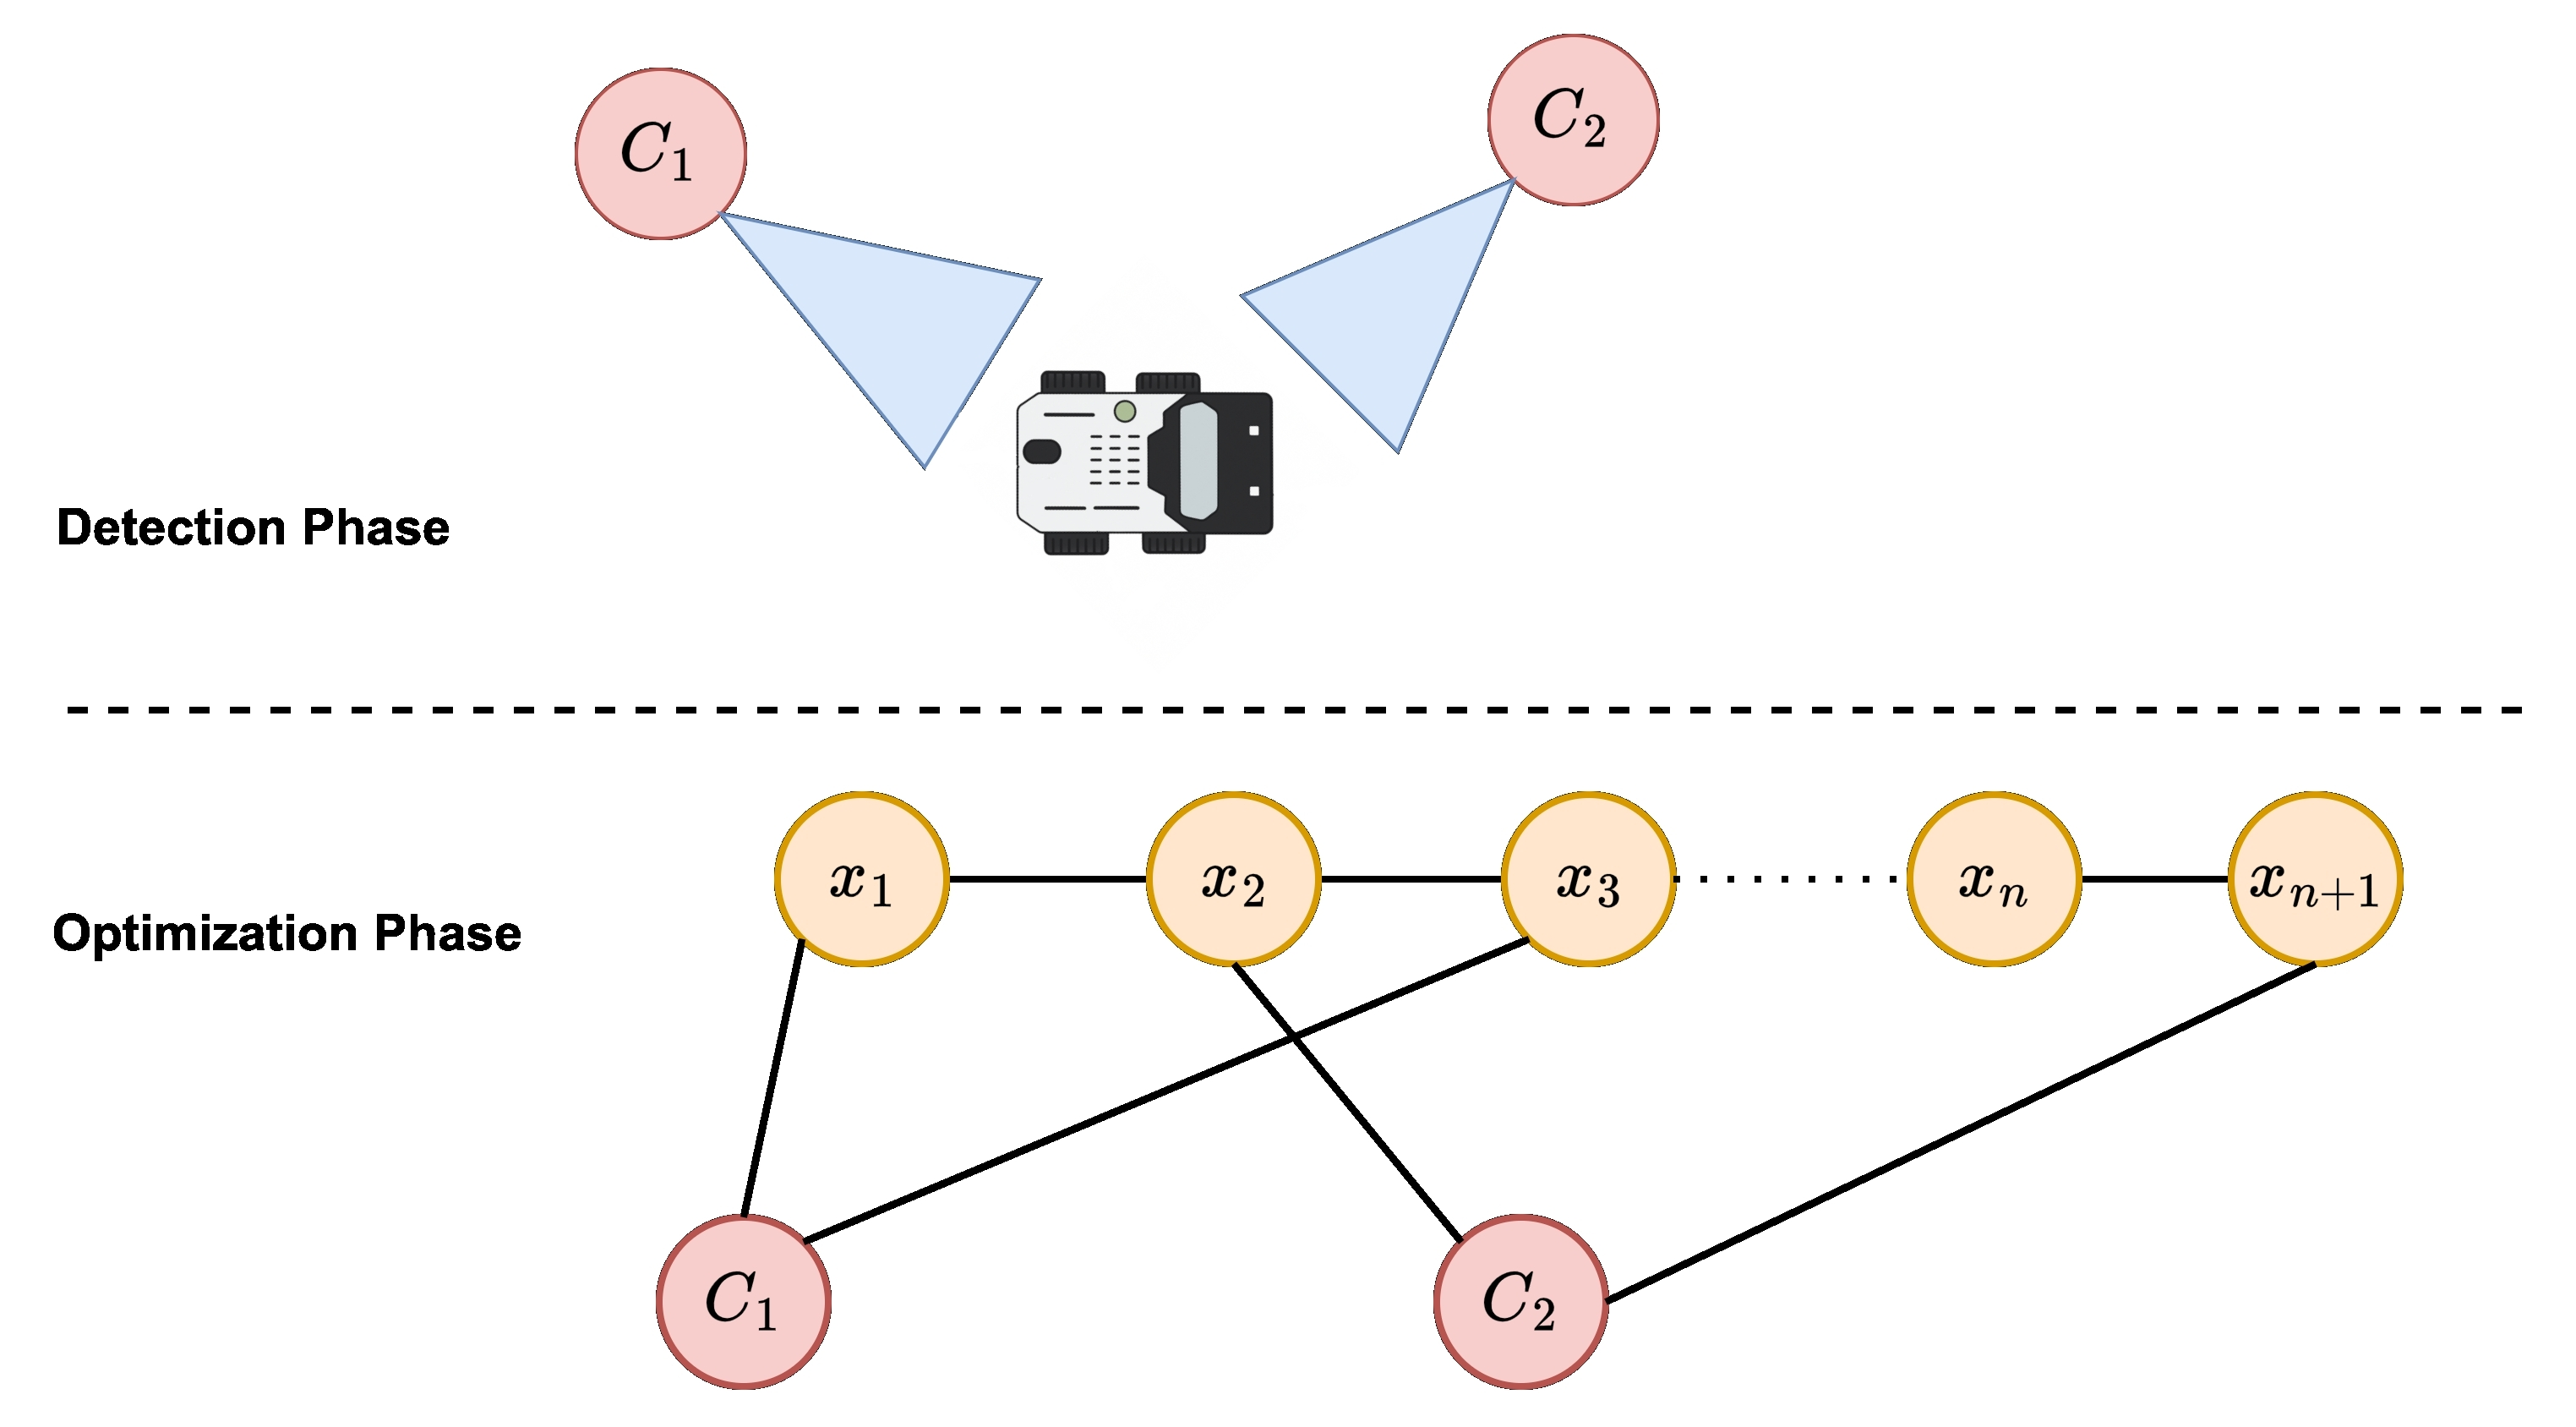
\includegraphics[width=\linewidth]{figures/architecture.jpg}
    \caption{Overview of the proposed framework. In the detection phase,
             fixed infrastructure cameras observe the robot from external
             viewpoints. In the optimisation phase, each observation adds a
             camera-to-robot relative pose constraint between a camera node
             $\mathcal{C}_i$ and a robot pose node $\mathbf{x}_t$, augmenting
             the LiDAR pose graph with repeated cross-time camera
             constraints.}
    \label{fig:system_overview}
\end{figure}

% ─────────────────────────────────────────────────────────────────────────
\subsection{Constraint Formulation}
\label{sec:constraint}

For each camera-derived anchor edge $(t,i) \in \mathcal{E}_{\mathrm{cam}}$,
the robot pose $\mathbf{x}_t$ is constrained relative to camera node
$\mathbf{x}_{\mathcal{C}_i}$.
The relative transform observed when the robot is detected is:

\begin{equation}
    \hat{\mathbf{T}}_{\mathcal{C}_i \to \text{robot}} =
        \mathbf{x}_{\mathcal{C}_i}^{-1} \cdot \mathbf{x}_t
    \label{eq:relative_transform}
\end{equation}

The associated camera residual, which instantiates the generic anchor residual
in Eq.~\ref{eq:pose_graph_objective}, is:

\begin{equation}
    \mathbf{r}^{\mathrm{cam}}_{ti}(\mathbf{x}_t, \mathbf{x}_{\mathcal{C}_i}) =
        \boldsymbol{\Sigma}_i^{-\frac{1}{2}}
        \left(
            \text{Log}\!\left(
                \hat{\mathbf{T}}_{\mathcal{C}_i \to \text{robot}}^{-1}
                \cdot \mathbf{x}_{\mathcal{C}_i}^{-1} \cdot \mathbf{x}_t
            \right)
        \right)
    \label{eq:residual}
\end{equation}

\noindent where $\boldsymbol{\Sigma}_i = \text{diag}(\sigma_x^2, \sigma_y^2, \sigma_\theta^2)$
encodes per-axis uncertainty and $\text{Log}(\cdot)$ is the $SE(2)$
logarithmic map.
This residual is inserted as a pose-camera term in the global objective,
penalizing inconsistency between the current robot pose estimate, the current
camera pose estimate, and the relative transform implied by the observation.
Because the same camera node participates in multiple detections collected at
different times, optimisation can refine that node jointly with the robot
trajectory instead of treating the camera as a pre-fixed absolute reference.

% ─────────────────────────────────────────────────────────────────────────
\subsection{Camera Node Initialisation and Refinement}
\label{sec:cam_init}

Each camera node is created lazily when that camera produces its first valid
detection of the robot.
Given the current robot estimate $\mathbf{x}_t$ and the observed relative
transform $\hat{\mathbf{T}}_{\mathcal{C}_i \to \text{robot}}$, an initial
map-frame estimate for the camera is obtained by inverting the measurement:

\begin{equation}
    \mathbf{x}^{(0)}_{\mathcal{C}_i} =
    \mathbf{x}_t \cdot
    \hat{\mathbf{T}}_{\mathcal{C}_i \to \text{robot}}^{-1}
    \label{eq:camera_init}
\end{equation}

This estimate is used only to initialise the parameter block and to associate
future observations with a persistent camera identity.
Every later detection from the same camera adds another residual of the form
in Eq.~\ref{eq:residual}, so the final camera pose is determined by the full
set of robot-camera observations together with the LiDAR odometry and
loop-closure constraints.
In this way, the cameras become anchor-like nodes through repeated geometric
consistency rather than through a manually entered pose on a completed map.

% ─────────────────────────────────────────────────────────────────────────
\subsection{Covariance Selection}
\label{sec:covariance}

The information assigned to each camera observation determines how strongly a
single detection can pull both the robot state and the associated camera node.
We therefore attach uncertainty to the relative measurement itself rather than
to a fixed map-frame camera prior.
In all experiments, we set $\sigma_x = \sigma_y = \SI{0.1}{\metre}$ and
$\sigma_\theta = \SI{0.05}{\radian}$, which provides a conservative weighting
for image-based robot localisation under pixel quantisation, projection error,
and partial occlusion.
This choice prevents one noisy detection from dominating the optimiser while
still allowing repeated observations from the same camera to accumulate into a
useful long-range constraint.
Sensitivity of the results to these values is analysed in
Section~\ref{sec:results}.

% ─────────────────────────────────────────────────────────────────────────
\subsection{Implementation}
\label{sec:implementation}

The inference node auto-discovers camera topics matching
\texttt{*/image\_raw} using periodic graph introspection.
Constraints are throttled to one per camera per \SI{5}{\second} to avoid
over-constraining the graph during bursts of detections.
The \texttt{add\_camera\_constraint} service extends the standard
Ceres-based SLAM problem in two ways.
When a camera is observed for the first time, the service allocates a new
camera parameter block initialised with Eq.~\ref{eq:camera_init}.
For every accepted detection, it adds a
\texttt{CameraConstraintFunctor} cost function implementing
Eq.~\ref{eq:residual} between the current robot pose node and that persistent
camera node.
In this way, the implementation realizes the graph augmentation described in
Eq.~\ref{eq:pose_graph_objective} without replacing the existing LiDAR SLAM
front-end or loop-closure pipeline, while allowing camera poses to be refined
online together with the map.
